\documentclass[12pt,oneside]{article}
\newcommand{\name}{Jean-Yves Djamen}
\newcommand{\class}{Math 80266A}
\newcommand{\hwnumber}{2}

\usepackage[margin=1in,letterpaper]{geometry}
%geometry changes the margins
%inside straight bracket is a parameter, inside curly bracket is name of package or whatever
%

\usepackage{amssymb,amsthm,amsmath,enumerate,fancyhdr,graphicx,tabularx}
\usepackage{float}
\usepackage{microtype}
\usepackage{tikz}
%Enables Graph Theory
\usepackage{pgfplots}
\usepackage{mdframed}
\usepackage[T1]{fontenc}
%Draws fancy boxes
\usepackage{parskip}
%Paragraph skip
\linespread{1.1} 
%Space in between lines
\usepackage{sectsty}
\sectionfont{\fontsize{12}{15}\selectfont}

\newenvironment{problem}[1]
{\begin{mdframed}
%Frames and crap
        \textbf{\textsc{Problem #1:}}
}
{\end{mdframed}}


\newenvironment{solution}
    {\textbf{\textsc{Solution:}}\\}
    {\newpage}

\pgfplotsset{compat=1.16}
\pagestyle{fancy}
\lhead{\textbf{\name}}
\chead{}
\rhead{\textbf{\class\ Assignment\ \hwnumber}}
\rfoot{\thepage}
\cfoot{}
\renewcommand{\headrulewidth}{0.2pt}

%lhead is the left header
%/textbf is text bold header

\def\l{\ell}
\def\pt{\partial}
\def\fish{\mathcal{I}}
\begin{document}

% \begin{enumerate}[I.]
% \item Solution number 1
% \item Solution Dos
% \item 
% \end{enumerate}

%/includgraphics

%/begin{align*}
%Stuff in here
%If star isn't included then the align command will automatically number your crap
%/end{align*}


\begin{problem}{1}
Simulate 1000 observations from each of the following data models. In each case, construct a Hill plot and comment.
\begin{enumerate}
    \item Consider an iid sequence with standard Cauchy marginal df.
    \item  Consider an iid sequence with standard Normal marginal df.
    \item Consider an AR(1) process $X_t = \phi X_{t-1} + Z_t$ where $\phi \in \{0.9, 0.5, 0.2\}$ and the noise sequence $\{Z_t\}$ comes from a symmetric distribution with exact Pareto tail $P(Z > x) =0.5x^{-10}$, $x \geq 1$. This yields $P(X > x) \sim cx^{-10}$.
\end{enumerate}
\end{problem}

\begin{solution}
We look now at several hill plots. Our goal is to notice a region of stability; preferably around small order statistics.
\section{Standard Cauchy}

We observe a region of stability around 1 which suggests the cauchy distribution has a tail index of 1.
\begin{figure}[H]
\begin{center}
{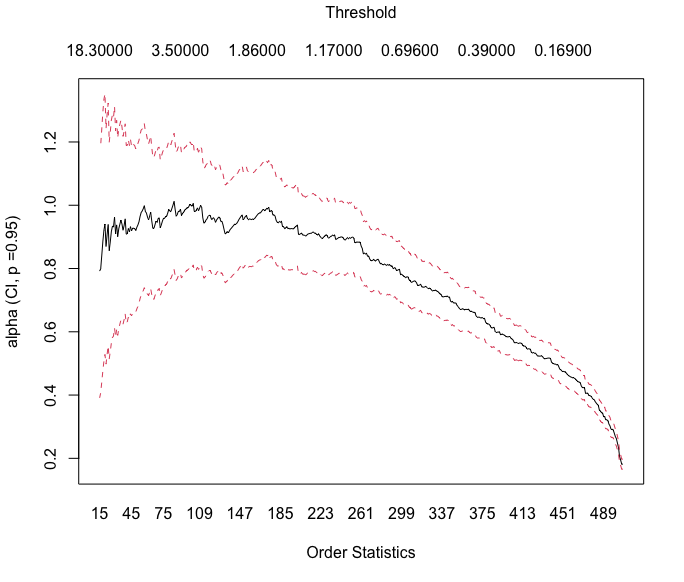
\includegraphics[width=3in]{Assignments/a3/hill-plot-cauchy.png}}
\caption{Hill plot for standard Cauchy distribution.}
\end{center}
\end{figure}

\section{Standard Normal}
Due to the intractability of the erf function, we expect condition (2) to not be completely satisfied, thus yielding an erratic and non-interpretable Hill plot.
\begin{figure}[H]
\begin{center}
{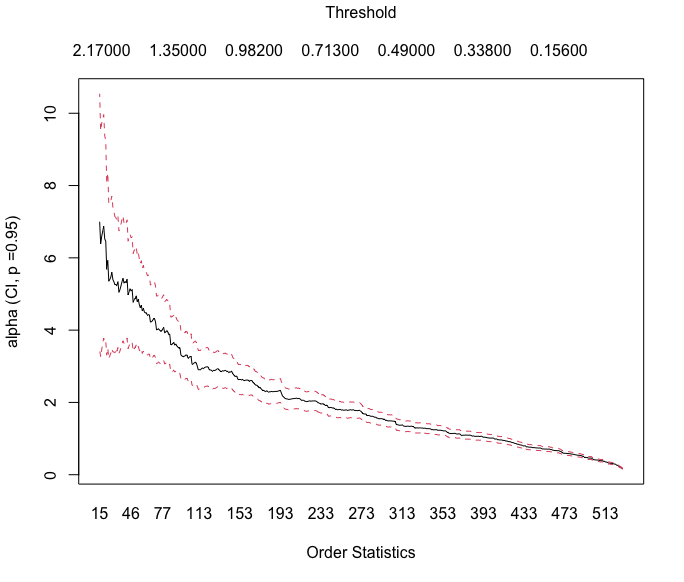
\includegraphics[width=3in]{Assignments/a3/hill-plot-normal.png}}
\caption{Hill plot for standard Normal distribution.}
\end{center}
\end{figure}

\section{AR(1) Processes}
First, we must recover the density function of the noise variable $Z_t$. Given that the sequence $\{Z_t\}$ is a symmetric distribution to be used as noise in an AR(1) process, as well as the right-sided behavior, we can sample points from $Z$.
\[P[Z\leq x] =\begin{cases} 1-0.5x^{-10} & x \geq 1 \\
0.5x^{-10} & x \leq -1 \end{cases}\]
Note that as $\{Z_t\}$ is to be used as a noise variable for an AR process, ensure that our cdf is symmetric around 0 and has an expectation of 0. Furthermore, we can invert the CDF and use uniform draws from (0,1) to sample from this sequence:
\[x=\begin{cases} [2(1-p)]^{\frac{-1}{10}} & \frac{1}{2}< p\leq 1\\
-([2p]^{\frac{-1}{10}}) & 0<p\leq \frac{1}{2}\end{cases}\]
Additionally, we are given that any AR(1) process we fit with this noise will have
\[P(X>x)\approx cx^{-10}\]
So, in the graphs below, we would hope to see a region of stability around $\hat{\alpha}=10$. However, the convergence of the Hill estimator hinges on the dependence of the sequence. We expect to see poor results for $\phi=0.9,0.5$ as the dependence between elements in these sequences can in no way be defined as ``weak". However, we hold out hope that at $\phi=0.2$ we will see a region of stability around $10$.
\subsection*{$\phi=0.9$}
In line with our assumptions, this Hill plot completely misses the true value of $\alpha$. 
\begin{figure}[H]
\begin{center}
{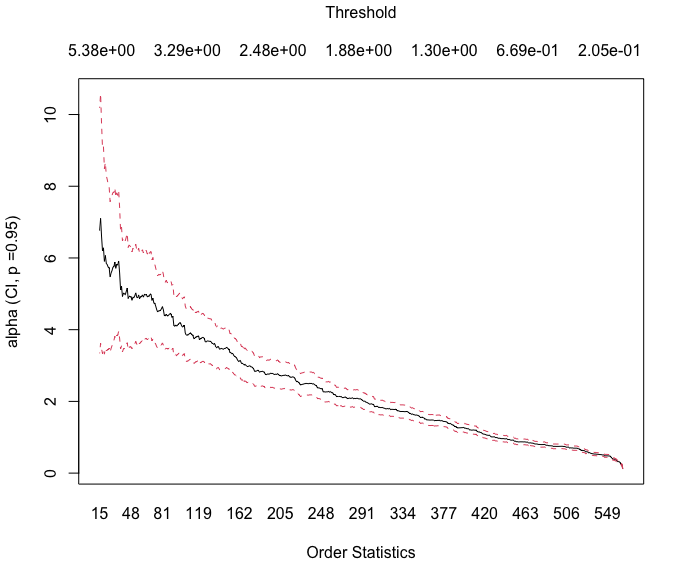
\includegraphics[width=3in]{Assignments/a3/hill-plot-ar9.png}}
\caption{Hill plot for AR(1) process with $\phi=0.9$.}
\end{center}
\end{figure}

\subsection*{$\phi=0.5$}
Although we observe more stable behavior around 10 (relative to $\phi=0.9$), we still note that the Hill plot is not stable enough around 10 to give an obvious reading. In fact, if we did not know the true underlying value of $\alpha$, we would be hard pressed to select 10 from analysis of the graph.
\begin{figure}[H]
\begin{center}
{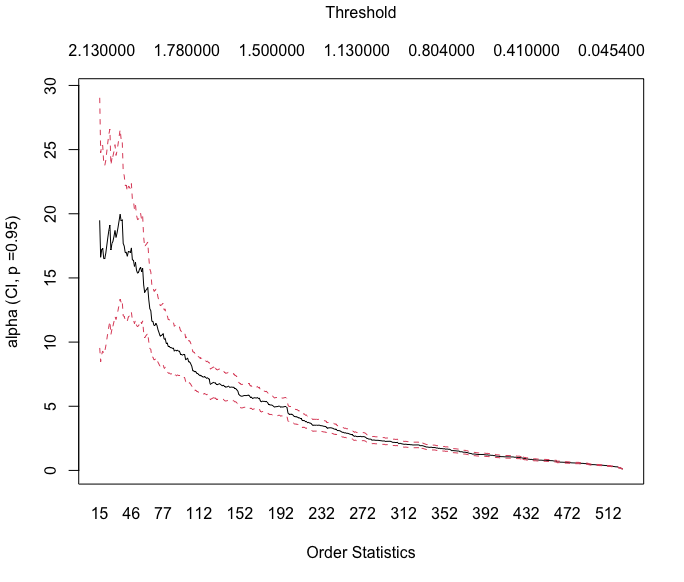
\includegraphics[width=3in]{Assignments/a3/hill-plot-ar5.png}}
\caption{Hill plot for AR(1) process with $\phi=0.5$.}
\end{center}
\end{figure}

\subsection*{$\phi=0.2$}
Here at least we see some stability. While $\hat\alpha$ seems to suggest a value around 12, this is the closest the Hill plot of our AR(1) experimental processes has gotten to the true value. However, we note that 10 is not in the confidence interval (starting from 112 ) which may suggest that the conditions on $k$ and $F$(for asymptotic normality of $\hat\alpha$) past this threshold are not satisfied.
\begin{figure}[H]
\begin{center}
{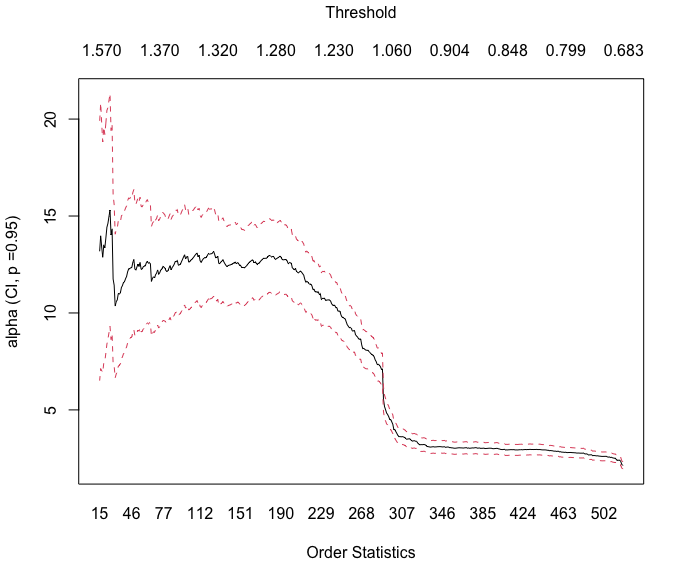
\includegraphics[width=3in]{Assignments/a3/hill-plot-ar2.png}}
\caption{Hill plot for AR(1) process with $\phi=0.2$.}
\end{center}
\end{figure}
\end{solution}

\begin{problem}{2}
We are interested in the maximum hourly rainfall in St. Louis, Missouri. The state of
Missouri suffered $\approx$ 3000 flash floods during 1996-2017, so clearly getting good estimates of the upper-tail behavior of hourly rainfall is crucial to building proper hydraulic structures and flood-protection infrastructure. 

\noindent In certain parts of the United States, rainfall is partially explained by the Southern Oscillation Index (SOI) and the Pacific Decadal Oscillation (PDO). Temperature can also partially explain precipitation. Changes over time are also possible due to climate change. Four data
files are supplied:
\begin{itemize}
    \item StLouis25.csv: hourly rainfall for months of April to August from 1979 to 2014 at a
location in St. Louis.
    \item SOIdata.csv: monthly SOI value from January 1951 to February 2020.
    \item PDOdata.csv: monthly PDO value from January 1854 to February 2020.
    \item MonthData-StLouis.csv: monthly weather statistics at St. Louis Lambert International Airport.
\end{itemize}
We focus on data for July and August. Analyzing the latter together or separately, produce useful estimates for monthly maximum hourly rainfall at this St. Louis location. Provide an executive summary of results, as well as a more detailed discussion referencing supporting
tables and figures.
\end{problem}

\begin{solution}
In our analysis, we use the supplied code to transform the hourly rainfall data into the max-monthly rainfall data. As we are looking for good estimates of the upper tail, we focus on the prediction of the $95^{th}$ and $99^{th}$ quantiles of the max rainfall data ($z_{0.05},z_{0.01}$). From our investigation, we found the best estimates and their confidence intervals below:
\begin{align*}
    p= 0.05 &&z_{0.05}\in [ , ] && \hat{z}_{0.05}= \\
    p= 0.01 &&z_{0.01}\in [ , ] && \hat{z}_{0.01}= 
\end{align*}
The methods for model creation, selection, and parameter estimation are discussed in the next sections.
\section*{Analyzing the data together}
We begin our analysis by considering July and August rainfall data as one dataset. This is done to lend more statistical power to our models through an increased number of observations. Latter analyses will consider the data separately. From observation of the data (shown below), we will assume that the monthly maximum hourly rainfall data follows a stationary process on which we can fit a covariate GEV. If the model diagnostics suggest this assumption is flawed, we will return to preprocessing the data to get declustered data that follow the $D(u_n)$ condition. The data, now assumed to be stationary, is shown below:
\begin{figure}[H]
\begin{center}
{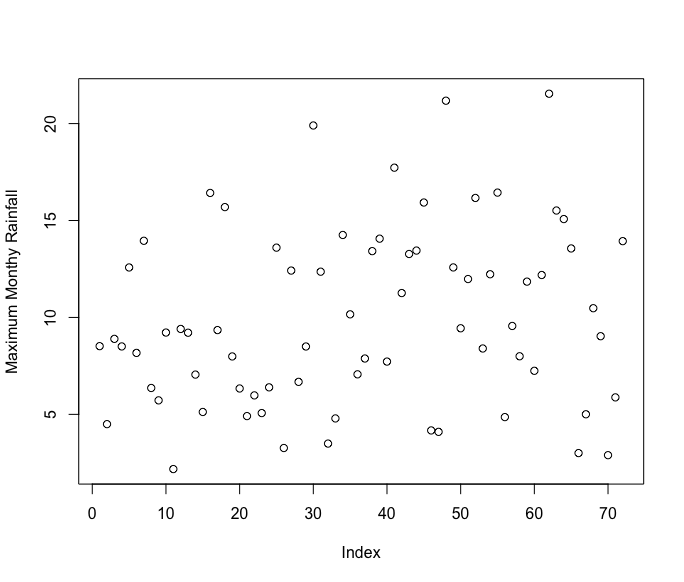
\includegraphics[width=3in]{Assignments/a3/rain.png}}
\caption{Maximum monthly rain}
\end{center}
\end{figure}
\noindent This decision made, we must decide which of the supplementary data we wish to include in our model. At a later point, this will be done through model selection. However, to get an intuitive feel for the data, we plot the monthly Saint Louis data against each of these covariates in turn.
\begin{figure}[H]
\begin{center}
{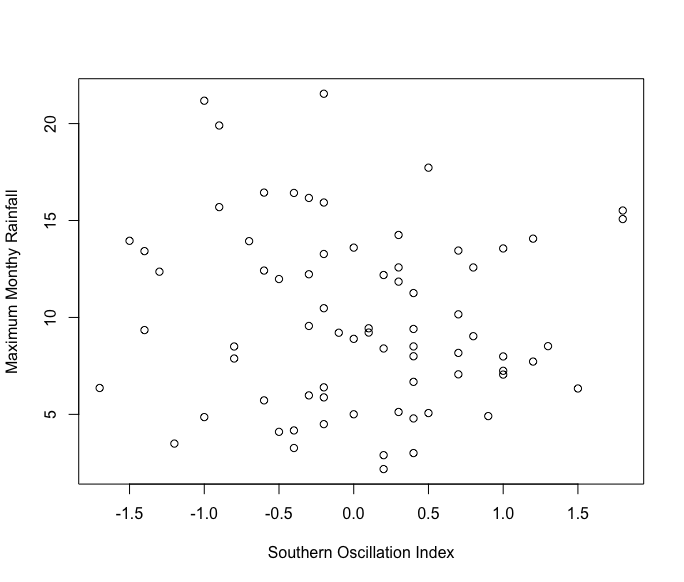
\includegraphics[width=3in]{Assignments/a3/rain-vs-soi.png}}
{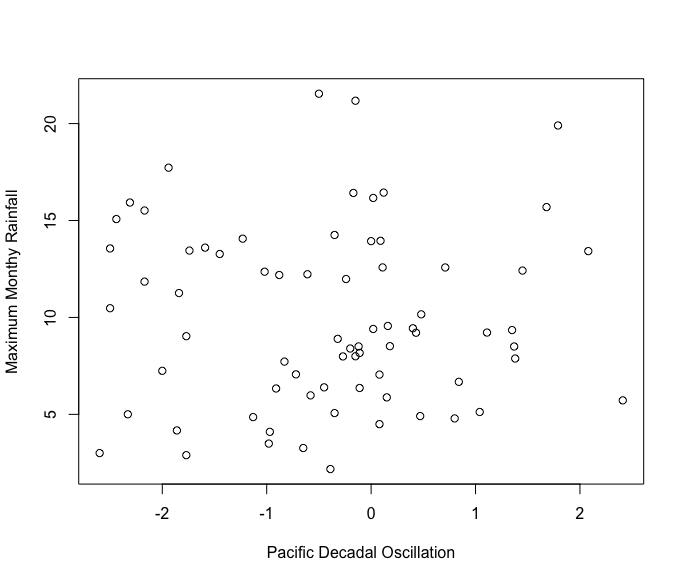
\includegraphics[width=3in]{Assignments/a3/rain-vs-pdo.png}}
{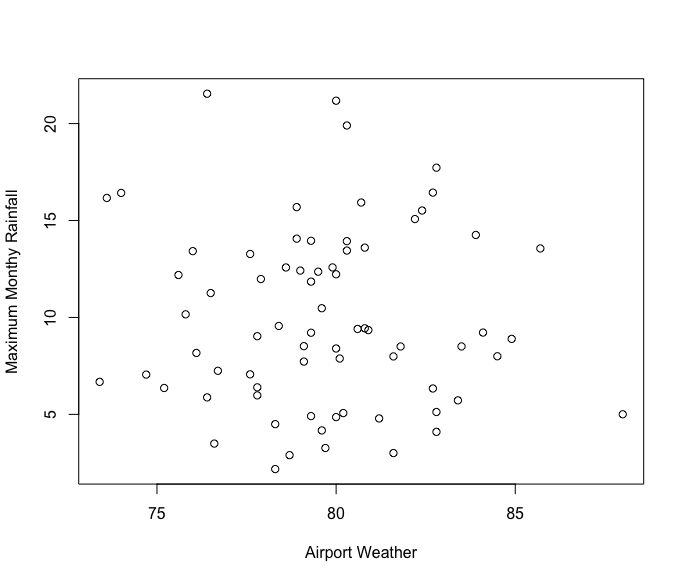
\includegraphics[width=3in]{Assignments/a3/rain-vs-temp.png}}
\caption{Maximum monthly rain plotted against potential covariates }
\end{center}
\end{figure}
\section*{Work}
Below is a complete list of models applied as well as their performance metrics (pp plots, qq plots, deviance). Models are indexed by the parameter chosen to be affected by the covariates:
\begin{align*}
    \text{Model I: }& \mu(t)=\beta_0+\beta_1\text{PDO}+\beta_2\text{SOI}+ \beta_3\text{TMP}\\
    \text{Model II: }& \mu(t)=\beta_0+\beta_1\text{PDO}+\beta_2\text{SOI}\\
    \text{Model III: }& \mu(t)=\beta_0+\beta_1\text{PDO}\beta_2\text{TMP}\\
    \text{Model IV: }& \mu(t)=\beta_0+\beta_1\text{SOI}+ \beta_2\text{TMP}\\
    \text{Model V: }& \mu(t)=\beta_0+\beta_1\text{PDO}\\
    \text{Model VI: }& \mu(t)=\beta_0+\beta_1\text{SOI}\\
    \text{Model VII: }& \mu(t)=\beta_0+\beta_1\text{TMP}\\
    \text{Model VIII: }& \mu(t)=\beta_0
\end{align*}
\end{solution}

\end{document}

